\documentclass[paper.tex]{subfiles}

\usepackage{tikz}
\usepackage{amsmath}
\usepackage{graphicx}
\usepackage{tabularx}
\usepackage{multicol}
\usepackage{algpseudocode}
\usepackage{algorithm}

\usepackage{setspace}

\usepackage{pgfplots}
\pgfplotsset{compat=1.16}

% Begin Document
\begin{document}

\section{Experimental Data}

Utilizing the two algorithms outlined above, we set out to test them with some randomized, undirected graphs.
We did this by generating random adjacency matrices.
Each node had a connection to itself for ease of comparsion.
Each node then had a chance to be connected to each other node, which we termed the graph density.
We used a value of $30\%$ for this graph density.

Then for each randomly generated graph, we ran both the brute force and approximation algorithms on it.
We did starting with a graph of 20 nodes, and ran these algorithms on a new randomized graph of incrementally larger size until the runtime exceeded 24 hours.
This happened at the 37-node mark with our implementation and hardware.
The data is below:

\singlespacing

\begin{center}
\begin{tabular}{c | r r | r r}

     & \multicolumn{2}{c |}{\textbf{Minimum Set}} & \multicolumn{2}{c}{\textbf{Approximate Set}} \\
     \textbf{\# of Vertices} & \textbf{Size} & \textbf{Time (seconds)} & \textbf{Size} & \textbf{Time (seconds)} \\ \hline

     20 &         4 &          0.46 &    7 &          8.6 e-6     \\
     21 &         4 &          1.00 &    5 &          6.5 e-6     \\
     22 &         4 &          2.09 &    5 &          6.6 e-6     \\
     23 &         4 &          4.46 &    7 &          9.2 e-6     \\
     24 &         4 &          9.44 &    8 &          1.0 e-5    \\
     25 &         5 &          20.15 &    7 &          9.6 e-6     \\
     26 &         5 &          42.07 &    5 &          8.9 e-6     \\
     27 &         4 &          90.59 &    6 &          1.0 e-5    \\
     28 &         4 &          233.23 &    8 &          1.2 e-5    \\
     29 &         4 &          395.63 &    8 &          1.2 e-5    \\
     30 &         4 &          852.31 &    7 &          1.3 e-5     \\
     31 &         4 &          1,834.03 &    7 &          1.4 e-5    \\
     32 &         4 &          3,869.44 &    6 &          1.4 e-5    \\
     33 &         4 &          8,145.86 &    6 &          1.4 e-5    \\
     34 &         4 &          17,353.50 &    7 &          1.5 e-5    \\
     35 &         5 &          35,943.60 &    10&          1.9 e-5   \\ 
     36 &         4 &          75,798.40 &    7 &          1.8 e-5  \\   
     37 &         4 &          161,439.00  &    8 &          2.0 e-5
    
\end{tabular}
\end{center}

\onehalfspacing

The doubling of the time needed to run each incrementally larger graph through the brute force algorithm is easily spotted in the data.
While a 37-node graph is not quite double the size of a 20-node graph, the time required ballooned from a half-second to nearly 45 hours.
As the trend will continue due to the nature of the brute force approach, we can extrapolate that a 38-node graph will take approximately 90 hours to compute the minimum set.
Further extrapolation reveals a 50-node graph will take over 42 \textit{years}.

On the other hand, the approximation algorithm ran near instantaneously for each graph, with its growth much lower.
The runtime of the approximation algorithm was measured in microseconds.
As is apparent, the approximation algorithm runs in orders of magnitude faster time than the brute force approach.

The question remains though, just how efficient is the approximation algorithm in terms of the size of the minimum set?
Below is a chart showing the relation between the minimum size and the approximate size for the data recorded above.

\vspace{5mm}

\begin{figure}[H]
\begin{center}
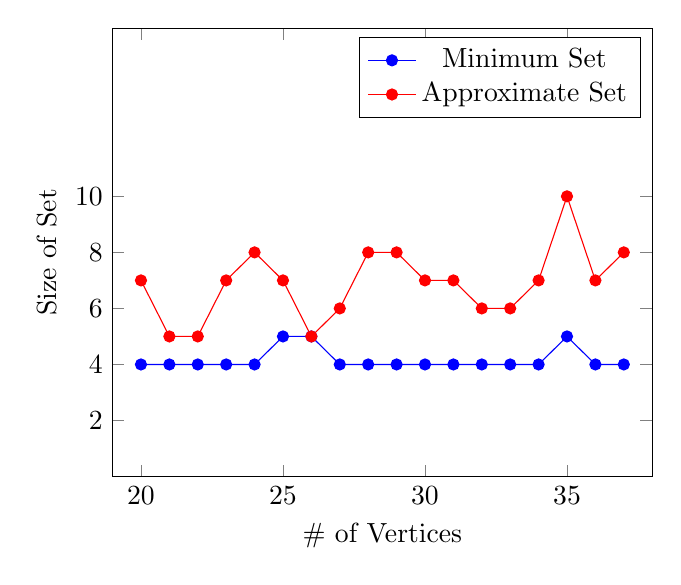
\begin{tikzpicture}
    \begin{axis}
        [
            xlabel = {\# of Vertices},
            ylabel = {Size of Set},
            xmin=19,xmax=38,
            ymin=0,ymax=16,
            xtick={20,25,30,35},
            ytick={2,4,6,8,10}
        ]

        \addplot[mark=*,blue] plot coordinates {
            (20,4)
            (21,4)
            (22,4)
            (23,4)
            (24,4)
            (25,5)
            (26,5)
            (27,4)
            (28,4)
            (29,4)
            (30,4)
            (31,4)
            (32,4)
            (33,4)
            (34,4)
            (35,5)
            (36,4)
            (37,4)
        };
        \addlegendentry{Minimum Set}

        \addplot[mark=*,red] plot coordinates {
            (20,7)
            (21,5)
            (22,5)
            (23,7)
            (24,8)
            (25,7)
            (26,5)
            (27,6)
            (28,8)
            (29,8)
            (30,7)
            (31,7)
            (32,6)
            (33,6)
            (34,7)
            (35,10)
            (36,7)
            (37,8)
        };
        \addlegendentry{Approximate Set}

    \end{axis}
\end{tikzpicture}
\end{center}
\end{figure}

As this chart shows, the approximate solution only found a minimum solution one time.
This indicates that it is entirely possible for the approximate solution to agree with the brute force approach.
However, the chart also clearly shows that the majority of cases in our test data were much larger than the minimal solution, often times double the size.

\end{document}